\documentclass[11pt,a4paper,headings=small,dvips]{scrbook}

\setcounter{secnumdepth}{3}
\setcounter{tocdepth}{3}
% This is used to create the cover and to plot trees
\usepackage{pst-tree}
\usepackage{pstricks,pstricks-add,multido}
%
\usepackage{geometry}
\usepackage{moresize}
%
%\usepackage{algorithmic}
% 
\usepackage{fancyvrb}
\usepackage{listings}
\usepackage{alltt}
\usepackage{gensymb}
% 
\usepackage{pbox}
% http://en.wikibooks.org/wiki/LaTeX/Indexing
\usepackage{makeidx} 
\makeindex
%
%\usepackage{subfigure}
% Figure caption settings
\usepackage[textfont=it,margin=10pt,font=small,labelfont=bf,labelsep=endash]{caption}
\usepackage{subcaption}
%
\usepackage{bm}
% Landscape package
\usepackage{lscape}
%
\usepackage{hyperref} 
\hypersetup{colorlinks=true}
\hypersetup{breaklinks=true}
% package for multiline comments
\usepackage{verbatim}
%
% Package to create a glossary - It must be uploaded after hyperref
% to produce the glossary: makeglossaries OQB
\usepackage[acronym,nonumberlist,style=altlist]{glossaries}
\glstoctrue
\makeglossaries
%
% - - - - - - - - - - - - - - - - - - - - - - - - - - - - - - - - Setting Fonts
\renewcommand{\encodingdefault}{OT1}
\renewcommand{\familydefault}{cmss}
\renewcommand{\seriesdefault}{m}
\renewcommand{\shapedefault}{up}

% - - - - - - - - - - - - - - - - - - - - - - - - - - - - - - - - - - - - - - -
\usepackage{amsmath}
% - - - - - - - - - - - - - - - - - - - - - - - - - - - - - - - - - - - - - - -
\usepackage{titlesec}
\usepackage[dvips]{graphicx}
% - - - - - - - - - - - - - - - - - - - - - - - - - - - - - - - - - - - - - - -
\usepackage{type1cm,eso-pic,color}

%\makeatletter
%\AddToShipoutPicture{
%    \setlength{\@tempdimb}{.5\paperwidth}
%    \setlength{\@tempdimc}{.5\paperheight}
%    \setlength{\unitlength}{1pt}
%    \put(\strip@pt\@tempdimb,\strip@pt\@tempdimc){
%        \makebox(0,0){\rotatebox{55}{
%        	\textcolor[gray]{0.85}{
%        		\fontsize{5cm}{5cm}
%        		\selectfont{DRAFT}}
%        	}
%        }
%	}
%}
%\makeatother

%
% Solves problems with margin notes
\usepackage{mparhack} 
	\setlength{\marginparwidth}{1.1in}
	\let\oldmarginpar\marginpar
	\renewcommand\marginpar[1]{\-\oldmarginpar[\raggedright\color{red01}
	\footnotesize #1]%
	{\raggedright\footnotesize #1}}
% Define some colors
	\definecolor{azure}{RGB}{240,255,255}
	\definecolor{honeydew}{RGB}{240,255,240}
	\definecolor{blue01}{RGB}{4,64,116}
	\definecolor{blue02}{RGB}{0,62,113}
	\definecolor{gray01}{rgb}{0.1,0.1,0.1}
	\definecolor{gray02}{rgb}{0.8,0.8,0.8}
	\definecolor{red01}{rgb}{0.5,0.0,0.0}
	\definecolor{orange00}{rgb}{1.0,0.74,0.53}
	\definecolor{orange01}{rgb}{0.9137,0.5882,0.0980}
	\definecolor{orange02}{rgb}{0.7608,0.4157,0.1804}
	\definecolor{orange03}{rgb}{0.6941,0.1843,0.1333}
\usepackage[english]{babel}
% Bibliography settings
\usepackage[square,colon]{natbib} % Extend bibligraphy functions
% Page numbering by Chapter
%\usepackage[auto]{chappg} 
%\pagenumbering{bychapter}
% 
% Define page properties
\usepackage{scrpage2}
	\pagestyle{scrheadings}
	\lofoot[]{
\includegraphics[width=2.0cm]{./figures/openquake_logo1.eps}}
	\refoot[]{
\includegraphics[width=2.0cm]{./figures/openquake_logo1.eps}}
	%\renewcommand{\partpagestyle}{empty}
% - - - - - - - - - - - - - - - - - - - - - - - - - -  Reformatting PART Titles
\titleformat{\part}[display]
{\filleft\normalfont\sffamily}
{\textcolor{blue01}{\bfseries\large PART}\hspace{4pt}
	\bfseries\Huge\textcolor{blue01}{\thepart}}
{1pc}
{\Huge\bfseries\textcolor{blue01}}
[]
% - - - - - - - - - - - - - - - - - - - - - - - - - Reformatting CHAPTER Titles
% Titles: CHAPTER
\titleformat{\chapter}
	[display] % shape
	{\filleft\normalfont\sffamily} % format
	{\textcolor{blue01}{\bfseries\MakeUppercase{\chaptertitlename}} % label
		\hspace{4pt}\huge\bfseries\textcolor{blue01}{\thechapter}} 
	{1pc} % sep
	{\huge\bfseries\textcolor{blue01}} % Before
	[]
% - - - - - - - - - - - - - - - - - - - - - - - - - Reformatting SECTION Titles
% Titles: SECTION
\titleformat{\section}
	[hang] % shape
	{\vspace{.8ex}\Large\bfseries\color{blue01}} % format 
	{\textcolor{blue01}{\thesection.}} % label
	{.5em} % sep
	{} % before
	[] % after
% - - - - - - - - - - - - - - - - - - - - - - -  Reformatting SUBSECTION Titles
% Title: SUBSECTION
\titleformat{\subsection}
	[hang] % shape
	{\vspace{.8ex}\large\bfseries\color{blue01}} % format 
	{\textcolor{blue01}{\thesubsection.}} % label
	{.5em} % sep
	{} % before
	[] % after
%  - - - - - - - - - - - - - - - - - - - - -  Reformatting SUBSUBSECTION Titles 
% Title: SUBSUBSECTION
\titleformat{\subsubsection}
	[hang] % shape
	{\vspace{.8ex}\normalfont\bfseries\color{blue01}} % format 
	{\textcolor{blue01}{\thesubsubsection.}} % label
	{.5em} % sep
	{} % before
	[] % after
% - - - - - - - - - - - - - - - - - - - - - - -  Reformatting PARAGRAPH Titles 
% Title: PARAGRAPH
\titleformat{\paragraph}
	[hang] % shape
	{\vspace{.2ex}\normalfont\color{blue01}} % format 
	{} % label
	{} % sep
	{} % before
	[] % after
%

\setcounter{secnumdepth}{2}
\setcounter{tocdepth}{2}

\usepackage{xcolor}
\usepackage{framed}

\newenvironment{myfancybox}{%
  \def\FrameCommand{\fboxsep=\FrameSep \fcolorbox{blue01}{honeydew}}%
  \color{black}\MakeFramed {\FrameRestore}}%
 {\endMakeFramed}

\setlength{\parskip}{2.5mm}
\setlength{\parindent}{0.0mm}

\begin{document}

\setcounter{page}{1}

\begin{titlepage}
	\title{ \textcolor{blue01}{\textsf{\bfseries\Huge 
        OpenQuake Training Workshop\\
        }}}
	\subtitle{ \textcolor{blue01}{\textsf{\bfseries\LARGE
        Cape Town, South Africa}}}
	\date{4 - 5 July 2012}
 
	\publishers{GEM Foundation, Pavia}
\end{titlepage}

\pagestyle{scrheadings}
\maketitle
\renewcommand*\thesection{\arabic{section}}
\renewcommand*\thefigure{\thesection.\arabic{figure}}
\clearpage
% -----------------------------------------------------------------------------
% -----------------------------------------------------------------------------
\chapter*{Introduction}
\cleardoublepage
% -----------------------------------------------------------------------------
% -----------------------------------------------------------------------------
\tableofcontents
\cleardoublepage
% -----------------------------------------------------------------------------
% -----------------------------------------------------------------------------
\chapter{Introduction to Openquake}
\begin{myfancybox}
The objectives of this chapter are:
\begin{itemize}
    \item aa
    \item bb
\end{itemize}
\end{myfancybox}
    % -----------------------------------------------------------------------------
\section{OpenQuake introduction}
% -----------------------------------------------------------------------------
\section{OpenQuake-hazard}
\subsection{Source typologies}
An OpenQuake PSHA input model contains a number of sources belonging 
to a finite set of possible typologies. Currently OpenQuake supports
four seismic source types. Each type contains a limited number of 
parameters necessary to specify geometry and seismicity occurrence.

OpenQuake, at present time, provides four seismic source typologies, 
for the most part defined in the GEM1 project \citep{pagani2010}. 
%
The main seismic source types currently supported are the following:
\begin{itemize}
\item Area source - So far, the most frequently adopted source 
type in national and regional PSHA models.
\item Grid sources - Grid sources can be considered a replacement 
for area sources since they both model distributed seismicity;
\item Simple fault - A Simple fault is the easiest way to
specify a fault source in OpenQuake. This typology is habitually adopted 
to describe shallow seismogenic fault sources.
\item Complex fault - A complex fault is more often used 
to model subduction interface sources with a complex geometry. 
\end{itemize}

These are the basic assumptions accepted in the definition of these source 
typologies:
\begin{itemize}
\item In the case of area and fault sources, the seismicity is homogeneously 
distributed over the source; 
\item Seismicity temporal occurrence follows a Poissonian model; 
\item The frequency-magnitude distribution distribution can be approximated 
to an evenly discretized distribution. 
\end{itemize}
%
%  . . . . . . . . . . . . . . . . . . . . . . . . . . . . . . . . . . . . . . . 
\subsubsection{Area sources}
\label{hazard:seismic_source_types:areaSources}
\index{Source type!area} 
\index{Area source|see{Source type}}
%
Area sources model the seismicity occurring over wide areas where  
identification or characterization - i.e. unambiguous definition 
of seismicity occurrence parameters - of single sources is difficult. 
%
The \citet{sshac1997} - using as a discriminant the extension - 
defined three main types of area seismic sources:
\begin{enumerate}
\item Area sources enclosing concentrated zones of seismicity;
\item Regional area sources;
\item Background area sources.
\end{enumerate}
%
The criteria adopted for their definition - and the related 
uncertainties - vary according to each area source type. 
%
From a computation standpoint we do not introduce any difference 
between these three area types.
%
%  . . . . . . . . . . . . . . . . . . . . . . . . . . . . . . . . . . . . . . . 
\paragraph{Parameters}
\begin{itemize}
\item A polygon that identifies the external border of the area. 
The current version of OQ doesn't support the definition 
of internal borders
\item One (or several) combinations of the following objects:
\begin{itemize}
	\item A discrete frequency-magnitude distribution 
	\item (optional) Strike, dip, and rake angles indicating 
	main fault geometry and slip direction for the seismicity  
	in the corresponding FMD.
	%
	For example, in the PSHA model prepared within the PEGASUS project,
	\cite{coppersmith2009} defines for each area source a discrete 
	distribution of strike values (dip is not considered because the 
	source-site metrics they use is the Joyner-Boore distance). 
\end{itemize}
%
This description permits the accurate characterization of seismicity 
occurrence within an area by explicitly taking into account the existing 
faulting trends. 
%
\item An array specifying the depth to the top of rupture dependency on 
magnitude. The array contains two columns and as many rows as the 
number of $<$depth, magnitude$>$ tuples used. 
The depth in each tuple defines the top of rupture for magnitudes equal 
or greater than the corresponding value. 
%
\item A value to indicate the hypocentral depth in case of punctual sources. 
By convention all the events with magnitude lower than the lowest value of 
magnitude contained in the depth to the top of rupture array are modelled as 
punctual sources. 
%
On the opposite, ruptures with magnitude equal or greater than 
the lowest value of magnitude contained in the depth to the top of rupture array 
are modelled considering their finite dimensions. The finite dimension of the 
rupture is computed using a magnitude-area or magnitude-length relationship 
specified in the calculation settings file (in future versions of OQ we will 
allow the user to specify for each tectonic region the corresponding 
magnitude-scaling relationship).
\end{itemize}
%
%  . . . . . . . . . . . . . . . . . . . . . . . . . . . . . . . . . . . . . . .
\subsubsection{Grid sources}
\label{hazard:seismic_source_types:gridSources}
\index{Source type!grid}
\index{Grid source|see{Source type}}
A grid source  is a typology used to model distributed seismicity - usually 
of low and intermediate magnitude.
%
Grid sources can be considered a PSHA source model alternative to area 
sources, since they both try to represent distributed seismicity. Grid sources 
usually derive from the application of seismicity smoothing algorithms 
\citep{frankel1995,woo1996}. 
%
The use of these algorithms carries some advantages compared to area sources, 
indeed, (1) they remove most of the unavoidable degree of subjectivity due to 
the definition of the geometries and (2) they define a seismicity spatial 
pattern that is, usually, more similar to reality. Nevertheless, some smoothing 
algorithms require the a-priori definition of some setup parameters that expose 
the calculation to a certain partiality level.

Grid sources are modelled in OpenQuake simply as a set of 
point sources. The next section describes the parameters required to 
characterize a point source.
%
%  . . . . . . . . . . . . . . . . . . . . . . . . . . . . . . . . . . . . . . . 
\paragraph{Parameters}
%
For each grid node:
\begin{itemize}
\item A location specified in terms of the $<$latitude,longitude$>$ tuple;
\item Similarly to area sources, one (or many) combinations of the following 
objects:
	\begin{itemize}
	\item A discrete frequency-magnitude distribution
	\item Strike, dip, and rake angles characterizing the seismicity 
	specified in the associated FMD. 
	\end{itemize}
\item An array to specify the dependency on magnitude of the depth to 
	the top of rupture. This array contains two columns and one or many 
	$<$depth, magnitude$>$ tuples where each tuple specifies the depth to the 
	top of rupture for magnitudes equal or greater than a specific value. 
\item A value to indicate the hypocentral depth in case of punctual sources. 
	The same convention specified for area sources applies here. 
\end{itemize} 
%
%  . . . . . . . . . . . . . . . . . . . . . . . . . . . . . . . . . . . . . . .
\subsubsection{Simple faults}
\index{Source type!fault!simple geometry} 
\index{Simple fault|see{Source type}}
%
Simple Faults are the most common source type used to model faults; the 
``simple'' adjective relates to the geometry description of the source 
which is basically obtained by projecting a trace (i.e. a polyline) along 
a representative dip direction. 
%
%  .   .   .   .   .   .   .   .   .   .   .   .   .   .   .   .   .   .   .   . 
\paragraph{Parameters}
%
\begin{itemize}
\item A fault trace (usually a polyline); 
\item A discrete frequency-magnitude distribution
\item A representative value of the dip angle (specified according to 
the Aki-Richards convention; see \citet{aki2002});
\item Rake angle (specified following the Aki-Richards convention; 
see \citet{aki2002}) 
\item Upper and lower values of depth limiting the seismogenic interval 
\item A boolean flag that specifies if the size of ruptures should 
follow a magnitude scaling relationship (currently specified in the 
calculation settings file) and be distributed homogeneously over the 
fault surface or it is accepted that ruptures within a given range of 
magnitudes (specified by the FMD) will always rupture the entire fault 
surface.
\end{itemize}
%
%  . . . . . . . . . . . . . . . . . . . . . . . . . . . . . . . . . . . . . . .
\subsubsection{Complex faults}
\index{Source type!fault!complex geometry}
\index{Complex fault|see{Source type}}
%
Complex faults  differ from simple fault just by the way geometry is 
described and, consequently in the way the fault surface is created. The 
input parameters used to describe complex faults are, for the most part, 
the same used to describe the simple fault typology. In particular, in 
the case of complex faults the dip angle is not requested while the fault
trace is substituted by two fault traces used to limit at top and bottom 
the fault surface. 
%
Usually, we use complex faults to model intraplate megathrust faults such 
as the big subduction structures active in the Pacific (Sumatra, South 
America, Japan).

% -----------------------------------------------------------------------------
\section{Calculation workflows}
% Three types of analysis
The hazard component of OpenQuake-Hazard performs seismic hazard 
analysis (SHA) following various approaches. 
%
Currently three main types of analysis are supported:
\begin{itemize}
\item \textit{Classical Probabilistic Seismic Hazard Analysis (cPSHA)}, 
allowing calculation of hazard curves and hazard maps following the 
classical integration procedure 
(\cite{cornell1968}, \citet{mcguire1976}) as formulated by \cite{field2003}).
\item \textit{Event-Based Probabilistic Seismic Hazard Analysis (ePSHA)}, 
allowing calculation of ground-motion fields from stochastic event sets. 
Eventually, classical cPSHA results - such as hazard curves - can be 
obtained by post-processing the set of computed ground-motion fields.
\item \textit{Deterministic SHA (DSHA)}, allowing calculation of ground 
motion fields from a single earthquake rupture scenario taking into account 
ground-motion aleatory variability.
\end{itemize}
Each of these analysis types has a modular structure, which provides the capability of investigating 
all possible intermediate results. Moreover, each calculator can be 
extended independently of the others so that more calculation 
options and methodologies can be easily introduced, without affecting the 
overall calculation workflow. 
Each of the workflows described in the following Sections involves a number 
of calculators, each responsible for a specific task. 
Figures \ref{classical_psha_workflow}, \ref{event_based_workflow}, and 
\ref{deterministic_workflow} schematically depict the different calculation 
workflows.
%
%  - - - - - - - - - - - - - - - - - - - - - - - - - - - - - - - - - - - - - - -
\subsection{Classical Probabilistic Seismic Hazard Analysis}
\label{section:classicalPSHA}
%
Input data for the classical PSHA consist of a PSHA Input Model (PSHAim) that 
is provided together with a set of calculation settings. 
%
The OpenQuake book \citep{crowley2011} describes extensively the content of 
a PSHAim and - in particular - the different options for modeling 
seismogenic sources and the option offered to include epistemic uncertainties 
on both seismicity and ground-motion models in the form of a logic tree.
%
% ..............................................................................
% . . . . . . . . . . . . . . . . . . . . . . . . . . . . . . . . . . . > Figure
\begin{figure}[htbp]
\begin{center}
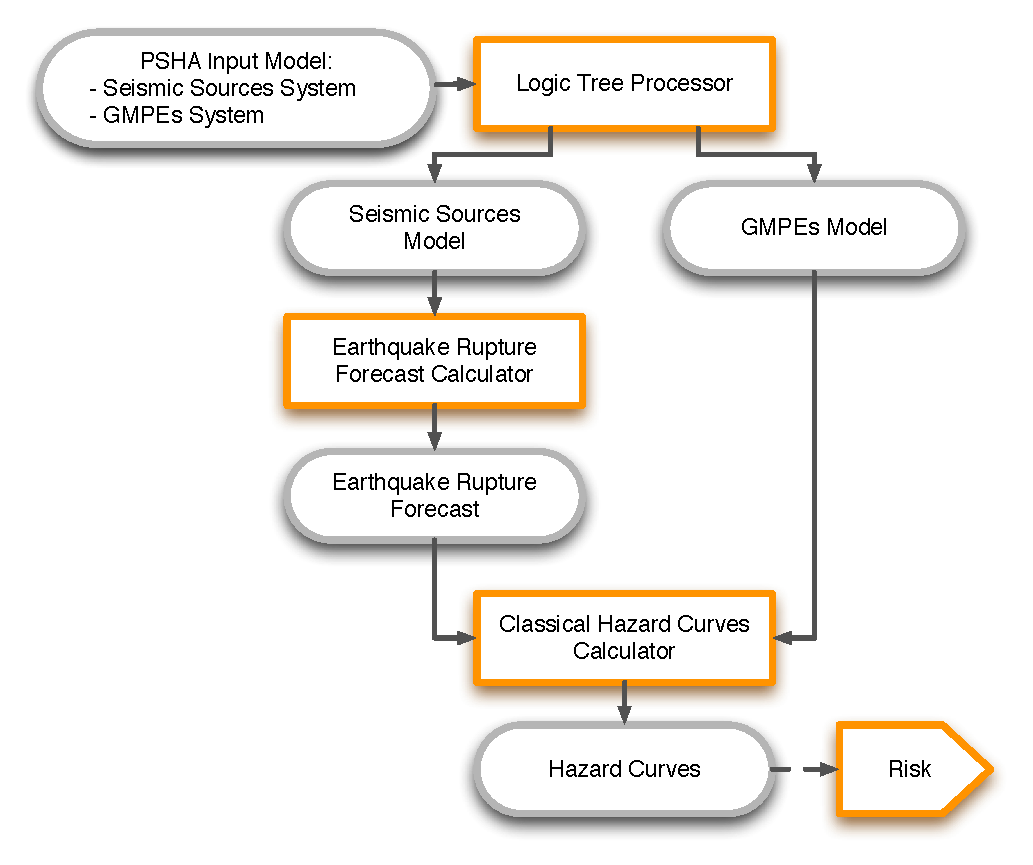
\includegraphics[width=14cm]{./figures/classical_psha_workflow.eps}
\caption{Workflow for classical PSHA (boxes with an orange border represent the 
calculators). Given a PSHA Input Model 
the Logic Tree Processor is responsible for creating a Seismic Source model
and a ground-motion model. 
The Seismic Source model is then provided to the Earthquake Rupture Forecast 
calculator, which computes the ERF (the list of all earthquake ruptures in the 
source model with their probabilities of occurrence). 
Using the ERF and the GMPEs model the Classical PSHA calculator produces 
curves at the sites of interest.}
\label{classical_psha_workflow}
\end{center}
\end{figure}
% . . . . . . . . . . . . . . . . . . . . . . . . . . . . . . . . . . . < Figure
% ..............................................................................

As represented in Figure \ref{classical_psha_workflow}, the main calculators 
used to perform this analysis are:
\begin{enumerate}
%
\item \emph{Logic Tree Processor} \hfill \\
The Logic Tree Processor (LTP) takes as an input the PSHA Input Model and 
creates a Seismic Source Model. The LTP uses the information in the Initial 
Seismic Source Models and by 'harvesting' the information contained in the 
Seismic Source Logic Tree - that is to sample the epistemic uncertainties - 
it creates a Seismic Source Model (i.e. a model describing geometry and 
activity rates of each source without any epistemic uncertainty). 
%
Following the procedure just described the Logic Tree Processor creates a 
Ground Motion model (i.e. a data structure that associates to each tectonic 
region considered in the calculation a GMPE).
%
\item \emph{Earthquake Rupture Forecast Calculator} \hfill \\
The produced Seismic Source Model is then used as input for the Earthquake 
Rupture Forecast (ERF) calculator which computes the probability of occurrence, 
over a specified time span, for each earthquake rupture produced by the source 
model.
\item \emph{Classical PSHA Calculator} \hfill \\
The cPSHA uses the ERF and the Ground Motion model to compute hazard curves on 
each site specified in the calculation settings.
\end{enumerate} 
%
%  - - - - - - - - - - - - - - - - - - - - - - - - - - - - - - - - - - - - - - -
\subsection{Event-Based Probabilistic Seismic Hazard Analysis}
\label{section:event-basedPSHA}
Input data for the Event-Based PSHA - as in the case of the Classical PSHA 
calculator - consist of a PSHA Input Model supplied to OQ together with a 
set of calculation settings.
%
% ..............................................................................
% . . . . . . . . . . . . . . . . . . . . . . . . . . . . . . . . . . . > Figure
\begin{figure}
\centering
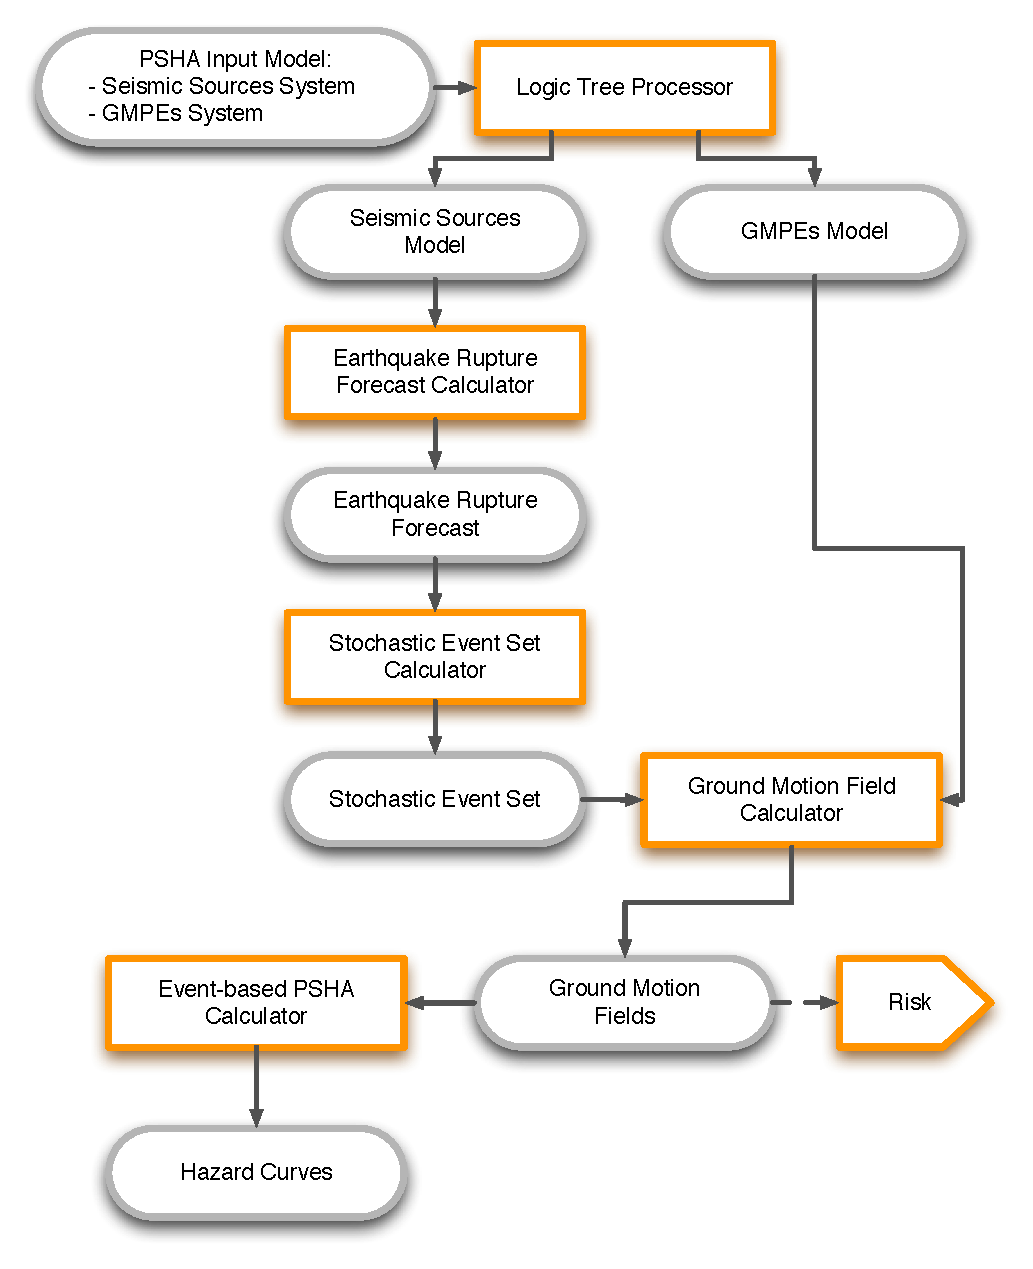
\includegraphics[width=14cm]{./figures/event_based_workflow.eps}
\caption{Workflow for event-based PSHA. Similar to the classical PSHA workflow 
(Figure \ref{classical_psha_workflow}), an ERF is computed, which is then used 
to generate a stochastic event set (representative of the seismic activity of 
a region in a given time span). Each event is then utilized to calculate a 
ground-motion field over a region of interest.}
\label{event_based_workflow}
\end{figure}
% . . . . . . . . . . . . . . . . . . . . . . . . . . . . . . . . . . . < Figure
% ..............................................................................
As represented in Figure \ref{event_based_workflow}, the main calculators 
used to perform this analysis are:
\begin{enumerate}
%
\item \emph{Logic Tree Processor} \hfill \\
The Logic Tree Processor was already 
introduced in the description of the cPSHA workflow (see section 
\ref{section:classicalPSHA} at page \pageref{section:classicalPSHA}).
%
\item \emph{Earthquake Rupture Forecast Calculator} \hfill \\ 
The Earthquake Rupture Forecast Calculator was already 
introduced in the description of the cPSHA workflow (see section 
\ref{section:classicalPSHA} at page \pageref{section:classicalPSHA}).
%
\item \emph{Stochastic Event Set Calculator} \hfill \\
The Stochastic Event Set Calculator generates a Stochastic Event set 
by sampling each rupture contained in the ERF according to its 
probability of occurrence. Usually a Stochastic Event Set (SES) contains
a large number of seismicity histories each one representative of a  
possible collection of events that can be produced by the seismic source
considered in an analysis during the time span fixed for the calculation
of hazard (normally corresponding to 50 years).
%
\item \emph{Ground Motion Field Calculator} \hfill \\
The Ground Motion Field Calculator computes for each event contained in a 
Stochastic Event Set - provided as an input - a realization of the 
ground shaking taking into account the aleatory uncertainties in 
the ground-motion model. Eventually, the Ground Motion Field calculator 
can consider the spatial correlation of the ground-motion during the 
generation of the GMF.
%
\item \emph{Event-based PSHA Calculator} \hfill \\
The event-based PSHA calculator takes a (large) set of ground-motion 
fields representative of the possible shaking that the investigated 
area can eventually experience over a (large) time span and for each 
grid node in a ground-motion fields computes the corresponding hazard 
curve. 
%
This procedure is computationally intensive and is not recommended for 
investigating the hazard over large areas. 
\end{enumerate}

The Logic Tree Processor and the Earthquake rupture forecast were already 
introduced during the descrption of the cPSHA workflow (see section 
\ref{section:classicalPSHA} at page \pageref{section:classicalPSHA}).
%
%  - - - - - - - - - - - - - - - - - - - - - - - - - - - - - - - - - - - - - - -
\subsection{Deterministic Seismic Hazard Analysis}
\label{section:deterministicSHA}
% Deterministic
For deterministic SHA (DSHA), the input data consist of a single earthquake 
rupture model and a single ground-motion model. Using the Ground Motion Field 
Calculator, multiple realizations of ground shaking can be computed, each 
realization sampling the aleatory uncertainties in the ground-motion model.

As represented in Figure \ref{deterministic_workflow}, the main calculators 
used to perform this analysis are:
\begin{enumerate}
\item \emph{Ground Motion Field Calculator} \hfill \\
The Ground Motion Field Calculator was already 
introduced during the descrption of the ePSHA workflow (see section 
\ref{section:event-basedPSHA} at page \pageref{section:classicalPSHA}).
\end{enumerate}
% ..............................................................................
% . . . . . . . . . . . . . . . . . . . . . . . . . . . . . . . . . . . > Figure
\begin{figure}[!hb]
\centering
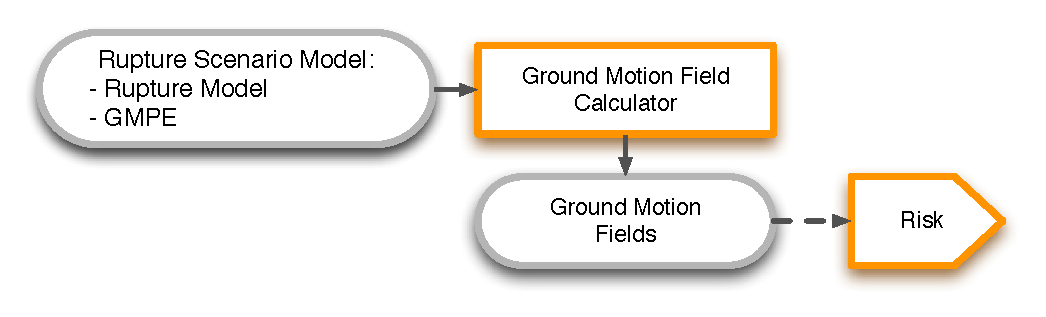
\includegraphics[width=14cm]{./figures/deterministic_workflow.eps}
\caption{Workflow for deterministic SHA. Given a rupture scenario model, 
consisting of an earthquake rupture model, plus a GMPE, the ground-motion 
field calculator can compute multiple ground-motion field realizations (by 
taking into account GMPE aleatory uncertainties).}
\label{deterministic_workflow}
\end{figure}
% ..............................................................................



\cleardoublepage

% -----------------------------------------------------------------------------
% -----------------------------------------------------------------------------
\chapter{Using Openquake}
\begin{myfancybox}
The objectives of this chapter are:
\begin{itemize}
    \item aa
    \item bb
\end{itemize}
\end{myfancybox}
    % -----------------------------------------------------------------------------
\section{Structure of an input model}

% -----------------------------------------------------------------------------
\section{Openquake demos}

\cleardoublepage

% -----------------------------------------------------------------------------
% -----------------------------------------------------------------------------
\chapter{Computing seismic hazard for Sub-saharan Africa using OpenQuake}
\begin{myfancybox}
The objectives of this chapter are:
\begin{itemize}
    \item Understand the basic input and output file structure
    \item Learn how to compute hazard curves and hazard maps
\end{itemize}
\end{myfancybox}
    \section{Model description}

The model used for this demo corresponds to the model proposed by 
\citet{midzi1999} in the context of the GSHAP project.

This seismic source model contains 21 area sources distributed within a wide 
band that goes from the Red Sea until South Africa.

\section{Assignment: hazard calculation using the demo model}
The first assignment focuses on the calculation of hazard for a small area 
using Openquake and demo model provided.

\subsection{Analysis of results}


\section{A brief demo of the Modeller's Toolkit - An African example}

The following will outline how to use the Modeller's Toolkit for the above example. In this exercise we shall be using the GSHAP area sources used in the previous demonstration, and utilising a new earthquake catalogue to recalculate the activity rates for the zones. This same process could be applied to any earthquake catalogue for the region and any area source zone model. 

\subsection{The Earthquake Catalogues}

Two earthquake catalogues are used for this exercise:
\begin{enumerate}
\item The Global CMT database (1976 - 2011) (Figure \ref{fig:Subsahara_Catalogue_GCMT_1})
\item A ''Homogenised'' Instrumental Catalogue - Derived from the ISC bulletin, converting the magnitudes from different agencies according to a hierarchical selection (Figure \ref{fig:Subsahara_Catalogue_ISC_1})
\end{enumerate}
\textbf{The ''Homogenised'' Catalogue has been created only for the purposes of the demonstration. There is NO ASSURANCE OF QUALITY and therefore the catalogue should NOT be used for any other purposes than demonstration!}

\begin{figure}[htbp]
	\centering
		\includegraphics[height=20cm, keepaspectratio=true]{./figures/Subsahara_Catalogue_GCMT_1.eps}
	\caption{Sub-Saharan Catalogue - GCMT}
	\label{fig:Subsahara_Catalogue_GCMT_1}
\end{figure}

\begin{figure}[htbp]
	\centering
		\includegraphics[height=20cm, keepaspectratio=true]{./figures/Subsahara_Catalogue_ISC_1.eps}
	\caption{Sub-Saharan Catalogue - ''New Homogenised''}
	\label{fig:Subsahara_Catalogue_ISC_1}
\end{figure}


\cleardoublepage

\section{Structure of an input model}
\section{Openquake demos}
\cleardoublepage
% -----------------------------------------------------------------------------
% -----------------------------------------------------------------------------
\chapter{Sub-saharan Africa demo}
The model used for this demo corresponds to the model proposed by 
\citet{midzi1999} in the context of the GSHAP project.
\section{Model description}
This seismic source model contains 21 area sources distributed within a wide 
band that goes from the Red Sea until South Africa.
\section{Assignment: hazard calculation using the demo model}
\subsection{Analysis of results}
\cleardoublepage
% -----------------------------------------------------------------------------
% -----------------------------------------------------------------------------
\chapter{Openquake-Modeller}
\begin{myfancybox}
The objectives of this chapter are:
\begin{itemize}
    \item aa
    \item bb
\end{itemize}
\end{myfancybox}
  The Hazard Modeller's Toolkit (or ''oq-hazard-modeller'') is a new development of the GEM OpenQuake suite, which is intended to provide scientists and engineers with the tools to help create the seismogenic input models that go into the OpenQuake hazard engine. The process of developing building the hazard model is a complex and often challenging one, and whilst many aspect of the practice are relatively common, the choice of certain methods or tools for undertaking each step can be a matter of judgement. The intention of this software is to provide scientists and engineers with the means to apply many of the most commonly used algorithms for preparing seismogenic source models using seismicitiy and geological data. It is still in an early stage of development and the current versions contain only a preliminary set of tools for undertaking the necessary workflows. In forthcoming versions will hope to make available more tools for the current processes indicated here, and to integrate new functionalities for i) merging and homogenisation of earthqake catalogues, ii) calculation of activity rates from geological and geodetic data, iii) testing and interpretation of Ground Motion Prediction Equations, and iv) integration of seismological and geological data and treatment of uncertainty in the construction of seismogenic source zones


\section{Getting Started and Running the Software}

The Modeller's Toolkit and associated software are designed for execution from the command line. As with OpenQuake, the preferred environment is Ubuntu Linux (11.04 or later). A careful effort has been made to keep the number of additional dependencies to a minimum. No packaged version of the software has been released at the time of writing, so the user must install the dependencies manually. The online documentation for the Modeller's Toolkit can be found at\\ \href{http://docs.openquake.org/mtoolkit}{http://docs.openquake.org/mtoolkit}.

\textbf{For the purposes of the current exercises all of the Modeller's Toolkit dependencies have been installed in both the OpenQuake .ova files and on the OATS server - so no installation is necessary! For instructions on how to install OpenQuake and the Modeller's Toolkit, please refer to the appendix of this document}

The execution of the Modeller's Toolkit is done from within the main directory in which the code is contained. The selection of the algorithm and the general configuration of the software is done via a configuration file (in this example \verb=config.yml=. This is a YAML (Yet Another Markup Language) file, which can be opened and edited with any common text editor (e.g. vi, emacs, gedit).

To run the Modeller's Toolkit simply move into the directory in which the \verb=main.py= file is found. Once the configuration file is correctly set up, execute via the following command:
\begin{Verbatim}[frame=single, commandchars=\\\{\}, fontsize=\scriptsize]
~\$ python main.py -i config.yml -d
\end{Verbatim}

The \verb=-d= indicates that the program can be run in ''debug'' mode. This will create a log (written automatically to the file \verb=debug.log=) of the processes that are executed inside the toolkit in addition to certain parameters that may be calculated at intermediate steps of the process, but are not written to the output. The \verb=-d= can be omitted if preferred, in which case the program will return only a minimal indication of the progress to the command prompt.


\subsection{The Configuration File}

The configuration file indicates to the toolkit where to look for input files, write output files, which processes and methods to apply and any possible parameters that should be set for given methods. A ''comprehensive'' example of the configuation file is given automatically in the file \verb=config.yml=, which outlines all possible options. The easiest process is to open this file, then edit and delete various options and parameters before saving the configution file to a new file (e.g. \verb=my_config_1.yml=) then executing that in place of the original configuration file. 

The various settings for the different algorithms will be discussed in due course, so the following considers just the main headers (i.e. the control) of the toolkit:

\begin{Verbatim}[frame=single, commandchars=\\\{\}, fontsize=\scriptsize]
\# *********************************************************
\# MT Workflow configuration file
\# *********************************************************
\\
\# =========================================================
\# Input/Output files
\# =========================================================
\\
\# Path to the file defining the eq catalog.
eq_catalog_file: tests/data/completeness_input_test.csv
\\
\# Path to the file defining the transformed
\# eq catalog after the preprocessing jobs.
\# If not defined no file will be written.
pprocessing_result_file: tests/data/preprocessed_catalogue.csv
\\
\# Path to the file defining the computed
\# completeness table after preprocessing jobs
completeness_table_file: tests/data/completeness_table.csv
\\
\# Path to the file defining the source model.
source_model_file: tests/data/area_source_model_processing.xml
\\
\# Path to the file defining the results
\# of computation.
result_file: tests/data/output.xml
\\
\# Boolean flag to declare
\# if processing jobs are needed.
apply_processing_jobs: yes
\\
\# =========================================================
\# List of preprocessing jobs
\# =========================================================
\\
\# Choose one algorithm per preprocessing job,
\# algorithms will be executed in the specified
\# order.
preprocessing_jobs:
- GardnerKnopoff
- Stepp
\\
\# =========================================================
\# List of processing jobs
\# =========================================================
\\
\# Choose one algorithm per preprocessing job,
\# algorithms will be executed in the specified
\# order.
processing_jobs:
- Recurrence
- MaximumMagnitude
\\
\# =========================================================
\# Preprocessing jobs in detail
\# =========================================================
\\
\# Declustering jobs
\\
.
.
.
\\
\# Completeness jobs
\\
.
.
.
\\
\# =========================================================
\# Processing jobs in detail
\# =========================================================
\\
\# Recurrence job
\\
.
.
.
\\
\# Maximum Magnitude Job
\\
.
.
.
\end{Verbatim}

In the initial lines, the toolkit is told the path to look for the input earthquake catalogue (\verb=eq_catalog_file=); the path to which it should write the ''pre-processed catalogue'' (\verb=pprocessing_catalog_file=); the path to which it should write the completeness table, or from which it should read the completeness table if no completeness jobs are defined (\verb=completeness_table_file=); the path from which it should find the area source geometries (\verb=source_model_file=), formatted here as xml (\verb=source_model_file=), and the path to write the output area sources (\verb=result_file=). 

The ''pre-processing'' refers to the combined operations for declustering and/or completeness - i.e. those that remove from consideration all events that are not indicative of complete stationary seismicity. If the user wishes to simply execute those jobs and no others then they should set the value \verb=apply_processing_jobs: no=. This will cause the program to terminate after completion of the pre-processing tasks. If the user has specified a valid path for the \verb=pprocessing_catalog_file= the program will export the catalogue with foreshocks, aftershocks and incomplete magnitude events removed.

After completion of the ''pre-processing'' tasks, the toolkit will then undertake the ''processing'' tasks. These are the calculations to determine the parameters of the double-truncated \cite{GutenbergRichter1944} distribution (i.e. a-value, b-value, minimum magnitude and maximum magnitude). If no source model input is specified in the \verb=source_model_file=, the processing will return (to the screen) a single a-value, b-value, $m_max$ and their respective uncertainties for the whole catalogue. Otherwise the program will loop over each of the zones specified in the file, select those earthquakes from the pre-processed catalogue that are found inside each zone and calculate the recurrence parameters for each zone. The output will then be written to the \verb=result_file=.

\textbf{The order in which the ''pre-processing'' and the ''processing'' tasks are define in the configuration is the order in which the program will execute them!}

\subsection{The Catalogue Format}

The input catalogue must be formatted as a comma-separated value file (.csv), with the following attributes (attributes with an * indicate essential attributes):

\begin{table}[h]
\begin{tabular}{|l|l|}  \hline 
Attribute & Description \\ \hline
eventID* & A unique identifier (integer) for each earthquake in the catalogue \\
Agency & The code (string) of the recording agency for the event solution  \\
Identifier & A secondary identifier (integer) not used at present  \\
year* & Year of event (integer) in the range -10000 to present \\
 & (events before common era (BCE) should have a negative value)\\
month* & Month of event (integer)\\
day* & Day of event (integer) \\
hour* & Hour of event (integer) - if unknown then set to 0 \\
minute* & Minute of event (integer) - if unknown then set to 0 \\
second* & Second of event (float) - if unknown set to 0.0 \\
timeError & Error in event time (float) \\
longitude* & Longitude of event, in decimal degrees (float) \\
latitude* & Latitude of event, in decimal degrees (float) \\
SemiMajor90 & Length (km) of the semi-major axis of the 90 \% \\
            & confidence ellipsoid for location error (float) \\
SemiMinor90 & Length (km) of the semi-minor axis of the 90 \% \\
            & confidence ellipsoid for location error (float) \\
ErrorStrike & Azimuth (in degrees) of the 90 \% \\
            & confidence ellipsoid for location error (float) \\
depth* & Depth (km) of earthquake (float)\\
depthError & Uncertainty (as standard deviation) in earthquake depth (km) (float)\\
Mw* & Moment magnitude of event (float) \\
sigmaMw & Uncertainty (standard deviation) in moment magnitude of event (float) \\
Ms & Surface-wave magnitude of event (float)\\
sigmaMs & Uncertainty (standard deviation) in surface-wave magnitude of event (float)  \\
mb & Body-wave magnitude of event (float)\\
sigmamb & Uncertainty (standard deviation) in body-wave magnitude of event (float) \\
ML & Local magnitude of event (float)\\
sigmaML & Uncertainty (standard deviation) in local magnitude of event (float) \\ \hline
\end{tabular}
\caption{List of Attributes in the Earthquake Catalogue File (* Indicates Essential)}
\label{tab: EQCatalogueFormat}
\end{table}

\subsection{The Source Model Format}


\section{Declustering}

To identify Poissonian rate of seismicity, it is necessary to remove foreshocks/aftershocks/swarms from the catalogue. The Modeller's Toolkit contains, at present, two algorithms to undertakte this task, with more under development.

\subsection{\cite{GardnerKnopoff1974}}

The most widely applied simple windowing algorithm is that of \cite{GardnerKnopoff1974}. Originally conceived for Southern California, the method simply identifies aftershocks by virtue of fixed time-distance windows proportional to the magnitude of the main shock. Whilst this premise is relatively simple, the manner in which the windows are applied can be ambiguous. Four different possibilities can be considered (\cite{LuenStark2012}):

\begin{enumerate}
 
\item Search events in magnitude-descending order. Remove events if it is in the window of the largest event

\item Remove every event that is inside the window of a previous event, including larger events

\item An event is in a cluster if, and only if, it is in the window of at least one other event in the cluster. In every cluster remove all events except the largest

\item In chronological order, if the $i^{th}$ event is in the window of a preceding larger shock that has not already been deleted, remove it. If a larger shock is in the window of the $i^{th}$ event, delete the $i^{th}$ event. Otherwise retain the $i^{th}$ event.

\end{enumerate}

It is the first of the four options that is implemented in the current toolkit, whilst others may be considered in future.  The algorithm is capable if identifying foreshocks and aftershocks, simply by applying the windows forward and backward in time from the mainshock. No distinction is made between primary aftershocks (those resulting from the mainshock) and secondary or tertiary aftershocks (those originating due to the previous aftershocks); however, it is assumed all would occur within the window.

Several modifications to the time and distance windows have been suggested, which are summarised in \cite{vanStiphout2010}. The windows originally suggested by \cite{GardnerKnopoff1974} are approximated by:

\begin{equation} 
\mbox{distance (km)} = 10^{0.1238 M + 0.983}  \quad \mbox{time} = \begin{cases} 10^{0.032 M + 2.7389} & \text{if $M \geq 6.5$} \\ 10^{0.5409 M - 0.547} & \mbox{otherwise}  \end{cases}
\end{equation}

An alternative formulation is proposed by Gr\:unthal \cite{vanStiphout2010}:

\begin{equation} 
\mbox{distance (km)} = e^{1.77 + \left( {0.037 + 1.02 M} \right)^2}  \quad \mbox{time} = \begin{cases}   |e^{-3.95+ \left( {0.62 + 17.32 M} \right)^2}    & \text{if $M < 6.5$ } \\ 10^{2.8 + 0.024 M} & \text{otherwise}  \end{cases}
\end{equation}
A further alternative is suggested by \cite{Uhrhammer1986}
\begin{equation}
\mbox{distance (km)} = e^{-1.024 + 0.804 M} \quad \mbox{time} = e^{-2.87 + 1.235 M}
\end{equation}

A comparison of the expected window sizes with magnitude are shown for distance (\ref{fig: declus_wind_dist}) and time (\ref{fig: declus_wind_dist}).

\begin{figure}[htbp]
  \centering
  \begin{subfigure}
      \centering
      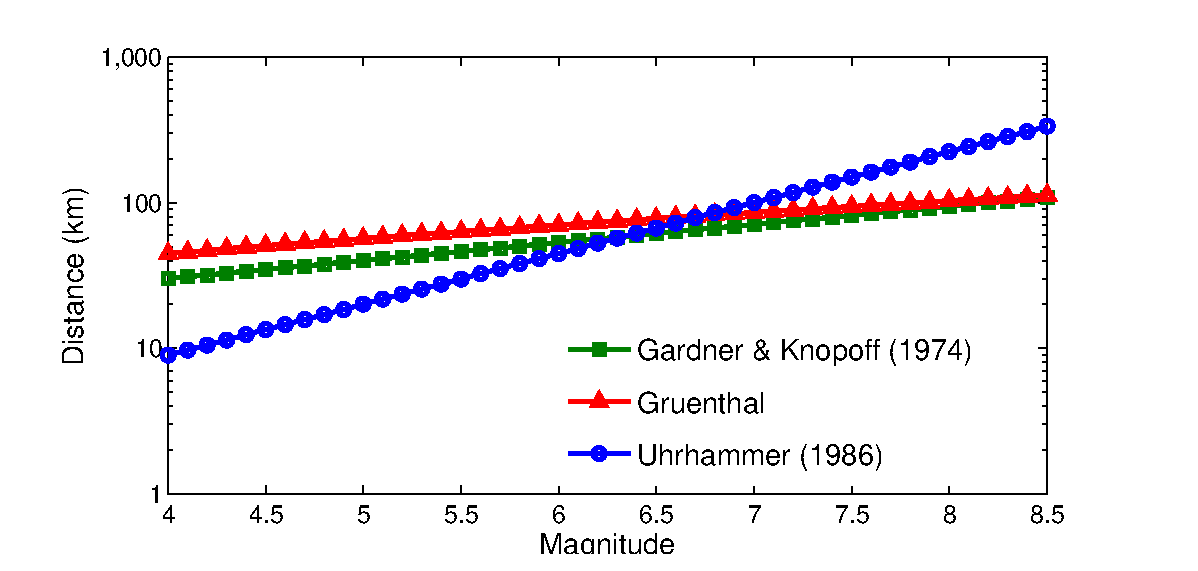
\includegraphics[width=8cm]{./figures/declustering_distance_windows.eps}
      %\caption{Distance (km)}
      \label{fig:declust_wind_dist}
	\end{subfigure}
	
  \begin{subfigure}
      \centering
      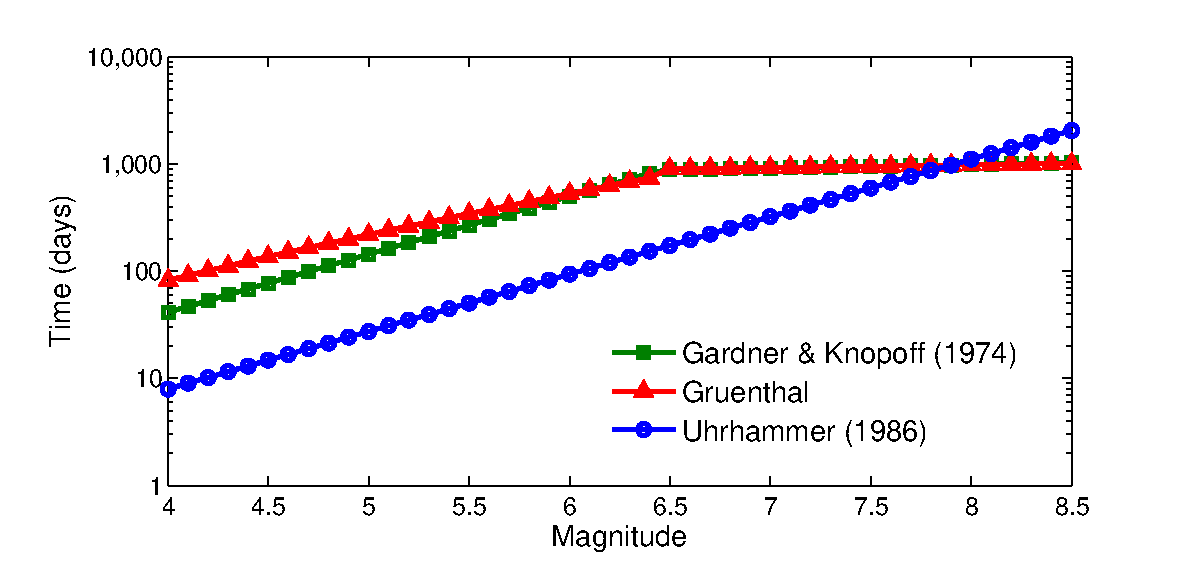
\includegraphics[width=8cm]{./figures/declustering_time_windows.eps}
      %\caption{Time}
      \label{fig:declust_wind_time}
	\end{subfigure}	
	\caption{Scaling of declustering time and distance windows with magnitude}
	\label{fig: declust_scaling}
\end{figure}

The \cite{GardnerKnopoff1974} algorithm and its derivatives represent are most computationally straightforward approach to declustering. Whilst the windows themselves may be derived from judgement, the algorithm has been found to be surprisingly robust, with the resulting declustered catalogues often demonstrated to be Poissonian \cite{vanStiphout2010}. 

The \cite{GardnerKnopoff1974} algorithm in the Modeller's Toolkit is configured according to the following command:

\begin{Verbatim}[frame=single, commandchars=\\\{\}, fontsize=\scriptsize]
GardnerKnopoff: \{ \\
  \# Possible values: GardnerKnopoff, Uhrhammer, Gruenthal\\
  time_dist_windows: GardnerKnopoff,\\
\\
  \# float >= 0 proportion of aftershock time windows\\ 
  \# to use to search for foreshock.\\
  foreshock_time_window: 0\\
\}
\end{Verbatim}

The \verb=time_dist_windows= attribute indicates the choice of the time and distance window scaling model from the three listed. As the current version of this algorithm considers the events in a descending-magnitude order, the parameter \verb=foreshock_time_window= defines the size of the time window used for searching for foreshocks, as a fractional proportion of the size of the aftershock window (the distance windows are always equal for both fore- and aftershocks). So for an evenly sized time window for foreshocks and aftershocks, \verb=foreshock_time_window= should equal 1. For shorter or longer foreshock time windows this parameter can be reduced or increased respectively.

%\section{Reasenberg (1985)} � Code written, not implemented in MTK

\subsection{AFTRAN (\cite{Musson1999PSHABalkan})}

A particular development of the standard windowing approach is introduced in the program AFTERAN \cite{Musson1999PSHABalkan}. This is a modification of the \cite{GardnerKnopoff1974} algorithm, using a moving time window rather than a fixed time window. In AFTERAN, considering each earthquake in order of descending magnitude, events within a fixed distance window are identified (the distance window being those suggested previously). These events are searched using a moving time window of 100 days. For a given mainshock, non Poissonian events are identified if they occur both within the distance window and the initial time window. The time window is then moved, beginning at the last flagged event, and the process repeated. For a given mainshock, all non-Poissonian events are identified when the algorithm finds a continuous period of 100 days in which no aftershock or foreshock is identified. 

The theory of the AFTERAN algorithm is broadly consistent with that of \cite{GardnerKnopoff1974}. This algorithm, whilst a little more computationally complex, and therefore slower, than the \cite{GardnerKnopoff1974} windowing approach, remains simple to implement. 

The AFTERAN algorithm in the Modeller's Toolkit is configured according to the following:

\begin{Verbatim}[frame=single, commandchars=\\\{\}, fontsize=\scriptsize]
Afteran: \{\\
    \# Possible values: GardnerKnopoff, Uhrhammer, Gruenthal.\\
    time_dist_windows: Uhrhammer,\\
    \\
    \# float >= 0 \\
    \# Length (in days) of moving time window\\
    time_window: 60.0\\
\}
\end{Verbatim}

As with the \cite{GardnerKnopoff1974} function, the \verb=time_dist_windows= attribute indicates the choice of the time and distance window scaling model. The parameter \verb=time_window= indicates the size (in days) of the moving time window used to identify fore- and aftershocks. 

%::::::::::::::::::::::::::::::::::::::::::::::::::::::::::::::::::::::::::::::::::::::::::::::::::::::::::::::::::::::::::::::::::::::::::::::::::::::::::::::

\section{Completeness}

In the earliest stages of processing an instrumental seismic catalogue to derive inputs for seismic hazard analysis, it is necessary to determine the magnitude completeness threshold of the catalogue. To outline the meaning of the term ''magnitude completeness'' and the requirements for its analysis as an input to PSHA, the terminology of \cite{Mignan2010} is adopted. This defines the magnitude of completeness as the ''lowest magnitude at which 100 \% of the events in a space-time volume are detected (\cite{RydelekSacks1989, WoessnerWiemer2005})''. Incompleteness of an earthquake catalogue will produce bias when determining models of earthquake recurrence, which may have a significant impact on the estimation of hazard at a site. Identification of the completeness magnitude of an earthquake catalogue is therefore a clear requirement for the processing of input data for seismic hazard analysis.

It should be noted that this summary of methodologies for estimating completeness is directed toward techniques that can be applied to a ''typical'' instrumental seismic catalogue. We therefore make the assumption that the input data will contain basic information for each earthquake such as time, location, magnitude. We do not make the assumption that network-specific or station-specific properties (e.g., configuration, phase picks, attenuation factors) are known a priori. This limits the selection of methodologies to those classed as estimators of ''sample completeness'', which defines completeness on the basis of the statistical properties of the earthquake catalogue, rather than ''probability-based completeness'', which defines the probability of detection given knowledge of the properties of the seismic network (\cite{SchorlemmerWoessner2008}). This therefore excludes the methodology of (\cite{SchorlemmerWoessner2008}), and similar approaches such as those of \cite{Gomberg1991} and \cite{Felzer2008}

The current workflows assume that completeness will be applied to the whole catalogue, ideally returning a table of time-varying completeness. The option to explore spatial variation in completeness is not explicitly supported, but could be accommodated by an appropriate configuration of the toolkit.

\subsection{User-defined Table} - Currently Available

This is simply a filtering that will remove from further consideration any events outside of the completeness bounds defined by the user. The table represents the time variation in $M_C$ and can be input as a separate file (in comma-separated value format) in the following format.
\begin{Verbatim}[frame=single, commandchars=\\\{\}, fontsize=\scriptsize]
1990.0, 4.0\\
1960.0, 5.0\\
1900.0, 6.0\\
1700.0, 7.0\\
\end{Verbatim}

The left-hand column represents the earliest year at which the earthquake is complete at the corresponding magnitude in the right-hand column. \\
\textbf{Important: The values in the completeness file must be entered from most-recent to oldest!} 

\subsection{\cite{Stepp1971}}

This is one of the earliest analytical approaches to estimation of completeness magnitude. It is based on estimators of the mean rate of recurrence of earthquakes within given magnitude and time ranges, identifying the completeness magnitude when the observed rate of earthquakes above MC begins to deviate from the expected rate. If a time interval ($T_i$) is taken, and the earthquake sequence assumed Poissonian, then the unbiased estimate of the mean rate of events per unit time interval of a given sample is:

\begin{equation}
   \lambda = \frac{1}{n} \sum_{i = 1}^{n} T_i
\end{equation}

with variance $\sigma_{\lambda}^{2} = \lambda / n$. Taking the unit time interval to be 1 year, the standard deviation of the estimate of the mean is:

\begin{equation}
   \sigma_{\lambda} = \sqrt{\lambda} / \sqrt{T}
\end{equation}

where $T$ is the sample length. As the Poisson assumption implies a stationary process, $\sigma_{\lambda}$ behaves as $1/\sqrt{T}$ in the sub-interval of the sample in which the mean rate of occurrence of a magnitude class is constant. Time variation of $M_C$ can usually be inferred graphically from Stepp's [1971] analysis, as is illustrated in Figure {fig: SteppFigExample1}. In this example, the deviation from the $1/sqrt{T}$ line for each magnitude class occurs at around 40 years  for $4.5 < M < 5$, 100 years for $5.0  < M < 6.0$, approximately 150 years for $6.0 < M < 6.5$ and 300 years for $M > 6.5$. Knowledge of the sources of earthquake information for a given catalogue may usually be reconciled with the completeness time intervals.

\begin{figure}[htbp]
	\centering
		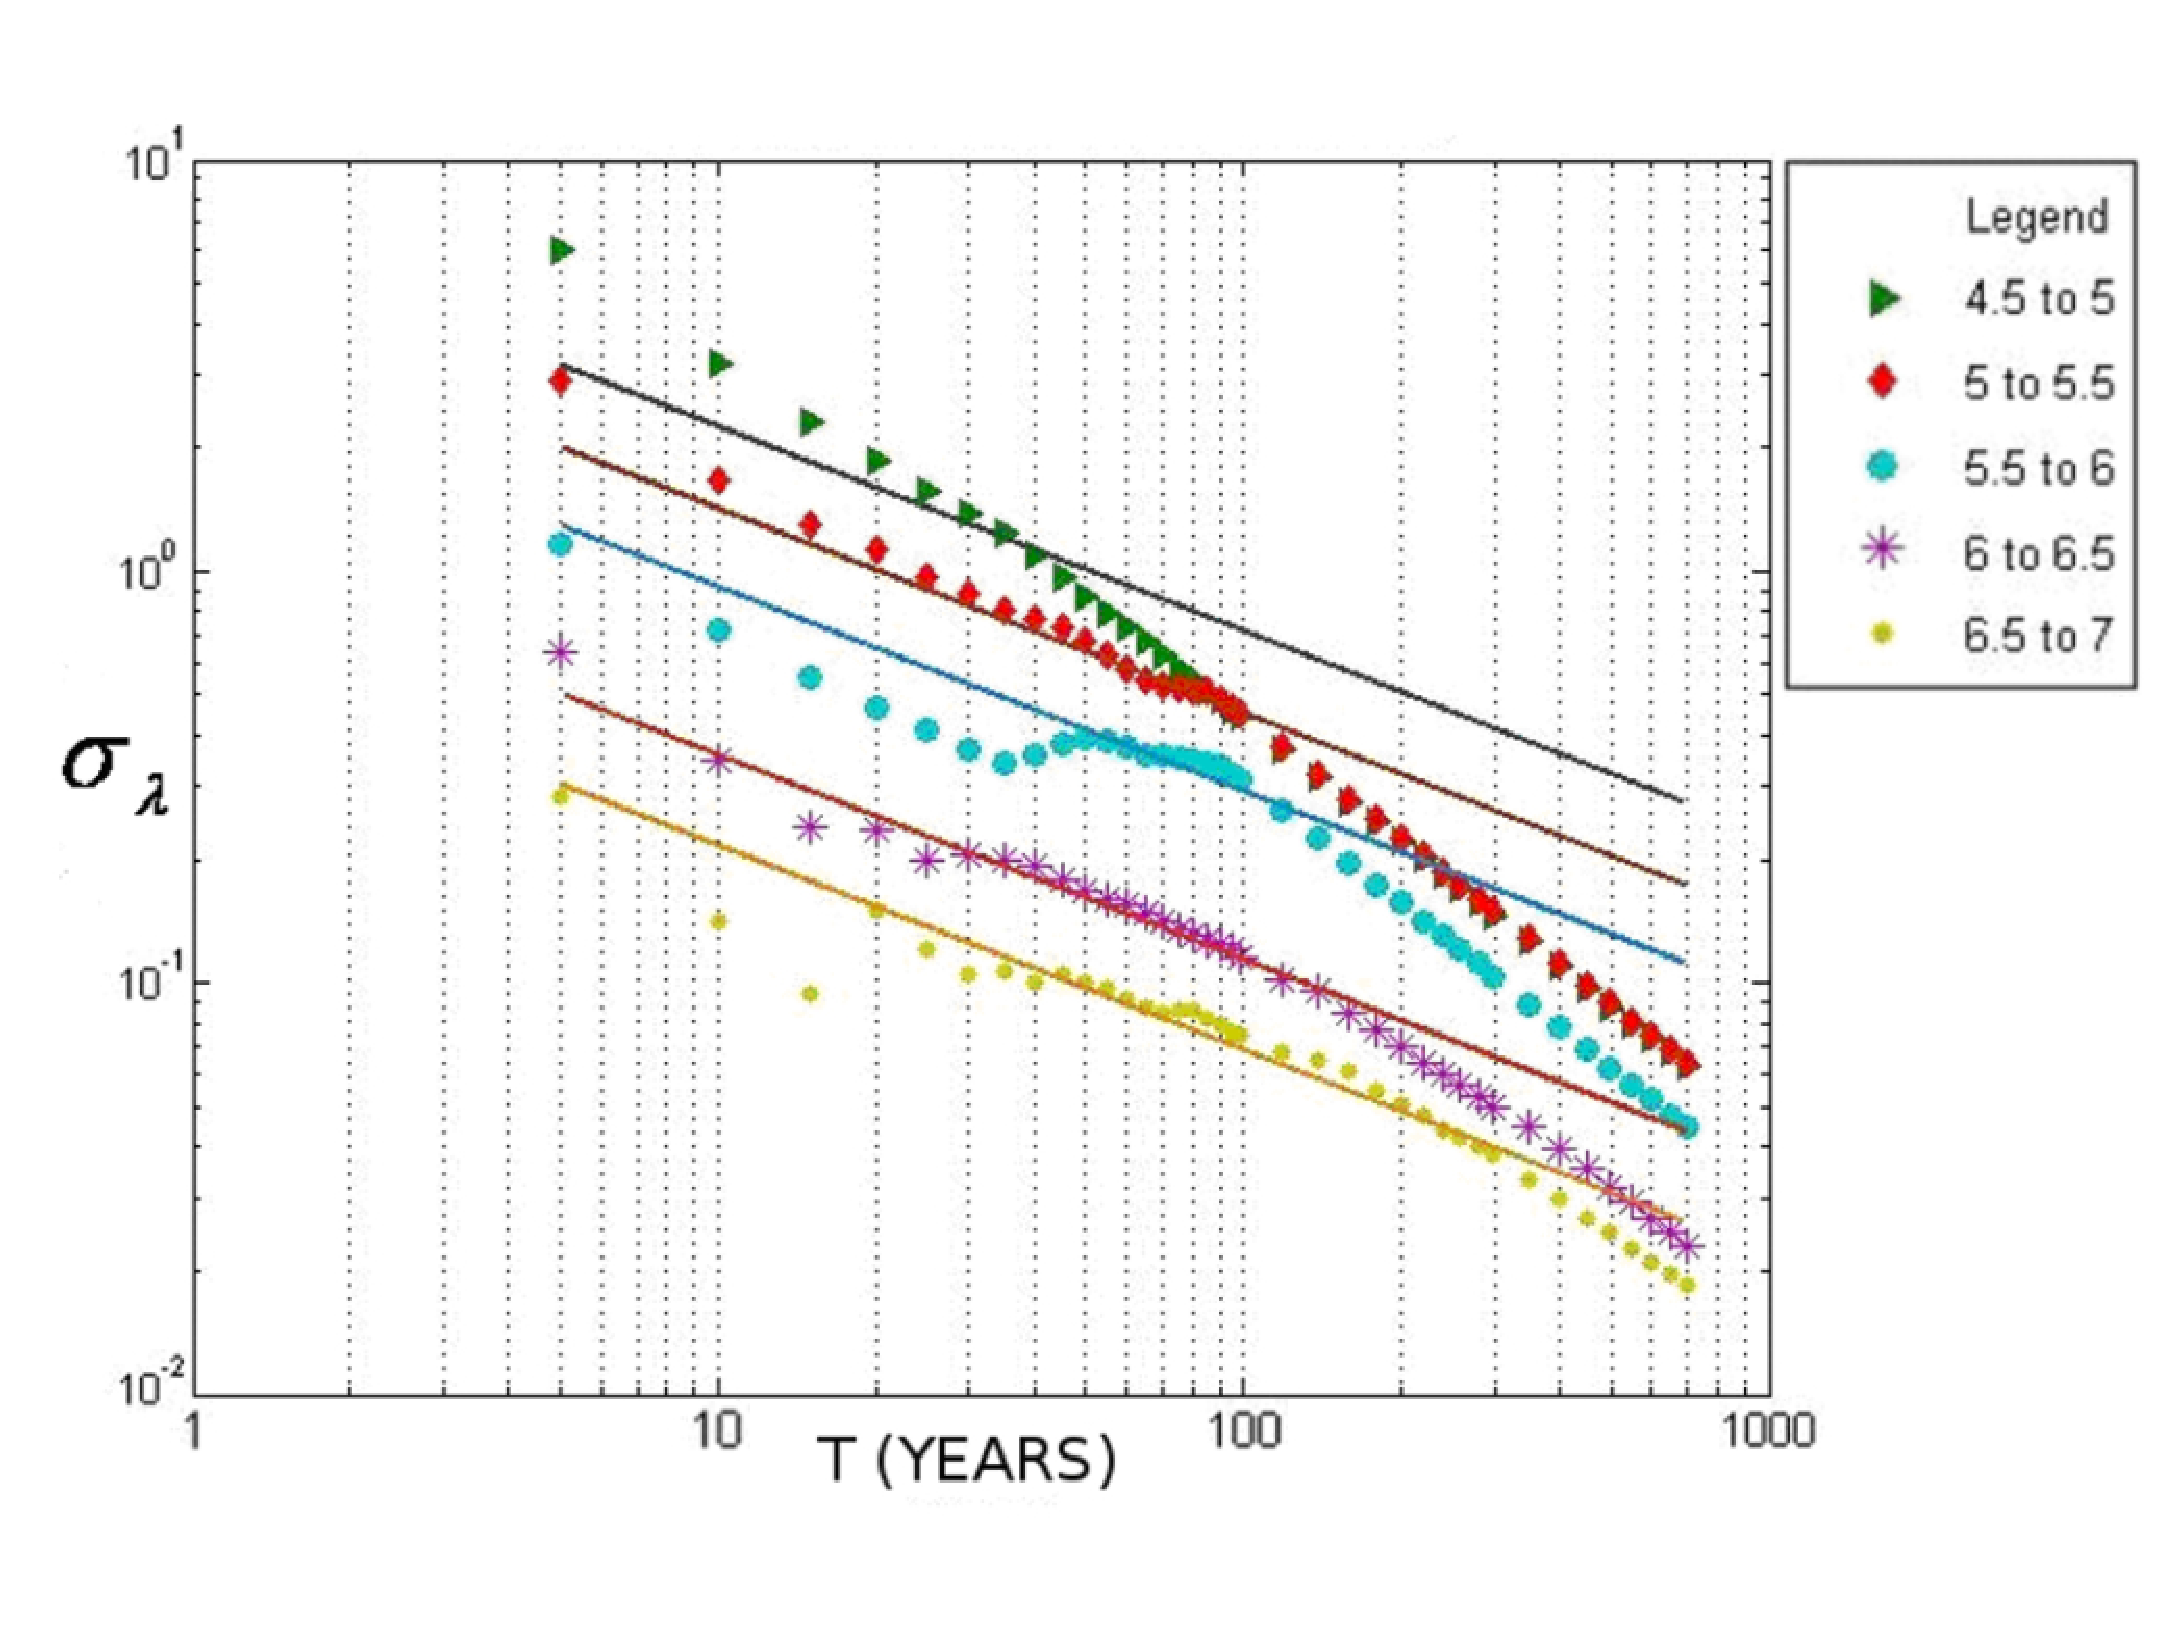
\includegraphics[height=10cm, keepaspectratio=true]{./figures/C2Fig1SteppFig1.eps}
	\caption{Example of Completeness Estimation by the \cite{Stepp1971} methodology}
	\label{fig:SteppFigExample1}
\end{figure}

The analysis of \citet{Stepp1971} is a coarse, but relatively robust, approach to estimating the temporal variation in completeness of a catalogue. It has been widely applied since its development. The accuracy of the completeness magnitude depends on the magnitude and time intervals considered, and a degree of judgement is often needed to determine the time at which the rate deviates from the expected values. It has tended to be applied to catalogues on a large scale, and for relatively higher completeness magnitudes. 

To translate the methodology from a largely graphical methods into a computational method the completeness period needs to be identified by automatically identifying the point at which the gradient of the observed values decreases with respect to that expected from a Poisson process. This divergence is identified by the second derivative of the line. Estimation of the precise time, however, can depend on what the user defines as an acceptable degree of divergence. To accommodate this, we define the parameter \verb=sensitivity=, which corresponds to a dimensionless value describing the degree of divergence. In most cases values between 0.05 and 0.2 are recommended.

In the current version of the Modeller's Toolkit only the \cite{Stepp1971} methodology for analysis of catalogue completeness is implemented. 

\begin{Verbatim}[frame=single, commandchars=\\\{\}, fontsize=\scriptsize]
Stepp: \{\\
  \# Time Window of each step (in years)\\
  time_window: 5,\\
\\
  \# Magnitude window of each step (in Mw units)\\
  magnitude_windows: 0.2,\\
  \\
  \# Sensitivity parameter (see documentation)\\
  sensitivity: 0.1,\\
  \\
  \# Increment Lock (fixes that the completeness magnitude\\
  \# will always increase further back in time)\\
  increment_lock: True \\
\} 
\end{Verbatim}

The \verb=time_window= parameter describes the size of the time window in years, the \verb=magnitude_window= parameter describes the size of the magnitude bin, sensitivity is as described previously. The final option (\verb=increment_lock=) is an option that is used to ensure consistency in the results to avoid the completeness magnitude increasing for the latest intervals in the catalogue simply due to the variability associated with the short duration. If \verb=increment_lock= is set to \verb=True=, the program will ensure that the completeness magnitude for shorter, more recent windows is less than or equal to that of older, longer windows. Otherwise it should be set to \verb=False to show the apparent variability=. Some degree of judgement is necessary here. In particular it is expected that the user may be aware of circumstances particular to their catalogue for which a recent increase in completeness magnitude is expected (for example, a certain recording network no longer operational).  


%::::::::::::::::::::::::::::::::::::::::::::::::::::::::::::::::::::::::::::::::::::::::::::::::::::::::::::::::::::::::::::::::::::::::::::::::::::::::::::::

\section{Recurrence Models}

The current sets of tools are intended to determine the parameters of the 
\subsection{Maximum Likelihood}

The classical maximum likelihood estimator for a simple unbounded \cite{GutenbergRichter1944} model is that of \cite{Aki1965}, adapted for binned magnitude data by \cite{Bender1983}. It assumes a fixed completeness magnitude ($M_C$) for the catalogue, and a simple power law recurrence model. It does not explicitly take into account magnitude uncertainty.


\begin{equation}
   b = \frac{ \log_{10} \left( e \right)}{ \bar{m} - m_0 + \left( {\frac{\Delta M}{2}} \right)}
\end{equation}

 We adjust for time-variation in completeness by divide the catalogue into S sub-catalogues, where each sub-catalogue corresponds to a period with a corresponding $M_C$. An �average� a- and b-value (with uncertainty) is returned by taking the mean of the a- and b-value of each sub-catalogue, weighted by the number of events in each sub-catalogue.

\begin{equation}
   \hat{b} = \frac{1}{S} \sum_{i = 1}^{S} w_i b_i
\end{equation}

\subsection{\cite{Weichert1980}}

Recognising the typical conditions of an earthquake catalogue, \cite{Weichert1980} developed a maximum likelihood estimator of $b$ for grouped magnitudes and unequal periods of observation. The likelihood formulation for this approach is:

\begin{equation}
   \mathbf{L} \left( {\beta | n_i, m_i, t_i} \right) = \frac{ N!}{\prod_i n_i!} \prod_i p_{i}^{n_i}
\end{equation}

where $\mathbf{L}$ is the likelihood estimator of $\beta$, $n$ the number of earthquakes in magnitude bin m with observation period t. The parameter $p$ is defined as:

\begin{equation}
   p_i = \frac{t_i \exp \left( {-\beta m_i} \right) }{\sum_j t_j \exp \left( {-\beta m_j} \right)}
\end{equation}

The extremum of $\ln \left( {\mathbf{L}}\right)$ is found at:

\begin{equation} 
   \frac{\sum_i t_i m_i \exp \left( {-\beta m_i} \right)}{\sum_j t_j \exp \left( {-\beta m_j} \right)}
\end{equation}

The computational implementation of this method is given as an appendix to \cite{Weichert1980}. This formulation of the maximum likelihood estimator for b-value, and consequently seismicity rate, is in widespread use, with applications in many national seismic hazard analysis \citep[e.g.]{usgsNSHM1996,usgsNSHM2002}. The algorithm has been demonstrated to be efficient and unbiased for most applications. It is recognised by \citet{Felzer2008} that an implicit assumption is made regarding the stationarity of the seismicity for all the time periods. 

To implement either of the recurrence estimators described here the configuration properties are defined as such:

\begin{Verbatim}[frame=single, commandchars=\\\{\}, fontsize=\scriptsize]
Recurrence: \{\\
    \# Width of magnitude window positive float\\
    magnitude_window: 0.2,\\
\\  
    \# Choose one among Weichert or MLE\\
    recurrence_algorithm: Weichert,\\
\\
    \# A float\\
    reference_magnitude: 5.0,\\
\\
    \# Greater than zero (float), used only with Weichert\\
    time_window: 1.0\\
\}
\end{Verbatim}

Where \verb=magnitude_window= indicates the size of the magnitude bin, \verb=recurrence_algorithm= the choice of the algorithm to use (either \verb=Weichert= or \verb=MLE=) and \verb=reference_magnitude= the magnitude for which the output calculates that rate greater than or equal to (set to \verb=0= for $10^{a}$). The \verb=time_window= indicates the bin of the time window used in the \cite{Weichert1980} algorithm. This value should generally be set to 1.0 for stability (the option to change it will be removed in future versions).


%::::::::::::::::::::::::::::::::::::::::::::::::::::::::::::::::::::::::::::::::::::::::::::::::::::::::::::::::::::::::::::::::::::::::::::::::::::::::::::::
\section{Maximum Magnitude}

The estimation of the maximum magnitude for use in seismic hazard analysis is a complex, and often controversial, process that should be guided by information from geology and the seismotectonics of a seismic source. Estimation of maximim magnitude from the observed (instrumental and historical) seismicity can be undertaken using the following non-parametric methods. These methods have been chosen from the possible ones available as they are intended to be independent of an assumption of the functional form of the recurrence model, and are therefore not conditioned upon b-value. 

\subsection{\cite{Kijko2004}}

Three different estimators of maximum magnitude are given by \cite{Kijko2004}, each depending on a different set of assumptions:
\begin{enumerate}
\item ''Fixed b-value'': Assumes a single b-value with no uncertainty (not considered here)
\item ''Uncertain b-value'': Assumes and uncertain b-value defined by an expected b and the standard deviation (not considered here)
\item ''Non-Parametric Gaussian'': Assumes no functional form (can be applied to seismicity observed to follow a more characteristic distribution)
\end{enumerate}

Whilst the fixed and uncertain b-value estimators can be applied in many situations, at present only the ''Non-Parametric Gaussian'' estimator is implemented here (the remainder will be implemented in due course).

The non-parametric Gaussian estimator for maximum magnitude $m_{max}$ is defined as:

%\begin{equation}
\begin{eqnarray}
m_{max} & = & m_{max}^{obs} + \Delta \\
\Delta  & = & \int\limits_{m_{min}}^{m_{max}} \left[ {\frac{\sum_{i = 1}^{n} \left[ {\Phi \left( {\frac{m - m_i}{h}} \right) - \Phi \left( {\frac{m_{min} - m_i}{h}} \right)} \right]}{\sum_{i = 1}^{n} \left[ {\Phi \left( {\frac{m_{max} - m_i}{h}} \right) - \Phi \left( {\frac{m_{min} - m_i}{h}} \right)} \right]}} \right]^n  dm
\end{eqnarray}
%\end{equation}
where $m_{min}$ and $m_{max}$ are the minimum and maximum magnitudes from a set of $n$ events, $\Phi$ is the standard normal cumulative distribution function. $h$ a kernel smoothing factor:
\begin{equation}
h = 0.9 \times min\left( {\sigma, IQR / 1.34} \right) \times n^{-1 / 5}
\end{equation}
with $\sigma$ the standard deviation of a set of n earthquakes with magnitude $m_{i}$ where $i = 1, 2, ... n$, and $IQR$ the inter-quartile range. 

The uncertainty on maximum magnitude is determined via:

\begin{equation}
    \sigma_{m_{max}} = \sqrt{\sigma_{m_{max}^{obs}}^2 + \Delta^{2}}
\end{equation}

Therefore the uncertainty on $m_{max}$ is conditioned primarily on the uncertainty of the largest observed magnitude. As in many catalogues the largest observed magnitude may be an earlier historical event, which will be associated with a large uncertainty, this estimator tends towards large uncertainties on $m_{max}$.



%\section{EPRI (1994), CEUS 2012} - Investigating

\subsection{\cite{MakropoulosBurton1983}} - Currently Available

\begin{Verbatim}[frame=single, commandchars=\\\{\}, fontsize=\scriptsize]
MaximumMagnitude: \{\\
    \# Choose one among `Kijko_Npg`, `Cumulative_Moment`.\\
    \# default choice: Cumulative_Moment,\\
    maxim_mag_algorithm: Kijko_Npg,\\
\\
    \# float > 0, default value 1.0E-5\\
    iteration_tolerance: 1.0E-5,\\
\\
    \# int > 0, default value 1000\\
    maximum_iterations: 1000,\\
\\
    \# neq\\
    neq: 100,\\
\\
    \# Used in Kijko_Npg\\
    \# int > 0 default value 51\\
    number_samples: 51,\\
\\
    \# Used in Cumulative_Moment\\
    \# int > 0 default value 100\\
    number_bootstraps: 100\\
\}
\end{Verbatim}
\cleardoublepage
% -----------------------------------------------------------------------------
% -----------------------------------------------------------------------------
\chapter{Improving the Sub-Saharan Africa demo model}
\begin{myfancybox}
The objectives of this chapter are:
\begin{itemize}
    \item aa
    \item bb
\end{itemize}
\end{myfancybox}
    \section{Catalogue processing}
\section{Calculation of activity rates}
\section{Assignment: Preparation of an updated OQ input demo model}
\subsection{Analysis of results}
\subsection{Comparison with previous results}

% -----------------------------------------------------------------------------
% -----------------------------------------------------------------------------
\cleardoublepage
\bibliographystyle{apalike}
\bibliography{./Bibliography/hazard}
\cleardoublepage
% -----------------------------------------------------------------------------
% -----------------------------------------------------------------------------
\end{document}
